% !TEX program = lualatex
% FORMAT AND PACKAGES
% {
\documentclass[a4paper, 11pt]{article}
\usepackage{a4wide,amssymb,epsfig,latexsym,multicol,array,hhline,fancyhdr}
% Vietnamese text (names on the title page): vntex with pdfLaTeX, native Unicode fonts with LuaLaTeX
\usepackage{iftex}
\ifLuaTeX
  \usepackage{fontspec}
\else
  \usepackage{vntex}
\fi
\usepackage{amsmath}
\usepackage{lastpage}
\usepackage[lined,boxed,commentsnumbered]{algorithm2e}
\usepackage{enumerate}
\usepackage{xcolor}
\usepackage{graphicx}							% Standard graphics package
\usepackage{array}
\usepackage{tabularx, caption}
\usepackage{multirow}
\usepackage{multicol}
\usepackage{rotating}
\usepackage{graphics}
\usepackage{geometry}
\usepackage{setspace}
\usepackage{epsfig}
\usepackage{tikz}
\usepackage{xfrac}
\usepackage{bm}
\usepackage{float}
\usepackage{subcaption}
\usepackage{listings}
\usepackage{mdframed}
\usepackage{booktabs}
\usepackage{needspace}
\usepackage[colorlinks]{hyperref}
\usepackage{xurl}
\definecolor{mauve}{rgb}{0.8, 0.4, 0.6}
\definecolor{dkgreen}{rgb}{0, 0.45, 0}
\lstset{frame=tb,
  language=C++,
  aboveskip=3mm,
  belowskip=3mm,
  showstringspaces=false,
  columns=flexible,
  basicstyle={\small \ttfamily},
  numbers=none,
  numberstyle=\tiny\color{gray},
  keywordstyle=\color{blue},
  commentstyle=\color{dkgreen},
  stringstyle=\color{mauve},
  breaklines=true,
  breakatwhitespace=true,
  tabsize=3, 
  numbers=left, numberstyle=\tiny,
}
\lstdefinelanguage{GLSL}[]{C++}{morekeywords={vec2,vec3,vec4,mat3,mat4,uniform,in,out,layout,sampler2D,location}}

% FORMATTING
% {
\DeclareMathOperator{\arccot}{arccot}
\captionsetup[table]{name=Table}
\captionsetup[figure]{name=Figure}
\newenvironment{Description}{\list{}{%
    \let\makelabel\descriptionlabel    % this comes from the original description environment
    \setlength{\rightmargin}{\leftmargin}% this comes from the original quote environment
    \setlength{\labelwidth}{0pt}%          this is new
    }}{\endlist}

\hypersetup{urlcolor=blue,linkcolor=black,citecolor=black,colorlinks=true} 
\usetikzlibrary{arrows,snakes,backgrounds,positioning,arrows.meta,shapes.geometric}
\definecolor{mathblue}{RGB}{0,114,188}
\newtheorem{theorem}{{\bf Theorem}}
\newtheorem{property}{{\bf Property}}
\newtheorem{proposition}{{\bf Proposition}}
\newtheorem{corollary}[proposition]{{\bf Corollary}}
\newtheorem{lemma}[proposition]{{\bf Lemma}}

\AtBeginDocument{\renewcommand{\listfigurename}{List of Figures}}
\AtBeginDocument{\renewcommand{\listtablename}{List of Tables}}
\AtBeginDocument{\renewcommand*\contentsname{Contents}}
\AtBeginDocument{\renewcommand*\refname{References}}

\setlength{\headheight}{40pt}
\pagestyle{fancy}
\fancyhead{} % clear all header fields
\fancyhead[L]{
 \begin{tabular}{rl}
    \begin{picture}(25,15)(0,0)
    \put(0,-8){\includegraphics[width=8mm, height=8mm]{hcmut.png}}
   \end{picture}&
	\begin{tabular}{l}
		\textbf{\bf \ttfamily University of Technology, Ho Chi Minh City}\\
		\textbf{\bf \ttfamily Faculty of Computer Science and Engineering}
	\end{tabular} 	
 \end{tabular}
}
\fancyhead[R]{
	\begin{tabular}{l}
		\tiny \bf \\
		\tiny \bf 
	\end{tabular}  }
\fancyfoot{} % clear all footer fields
\fancyfoot[L]{\scriptsize \ttfamily Computer Graphics - Academic year 2026 - 2027}
\fancyfoot[R]{\scriptsize \ttfamily Page {\thepage}/\pageref{LastPage}}
\renewcommand{\headrulewidth}{0.3pt}
\renewcommand{\footrulewidth}{0.3pt}

\setcounter{secnumdepth}{3}   % (template: 4) so that \paragraph headings stay unnumbered
\setcounter{tocdepth}{2}      % (template: 4) sections and subsections only in the contents

\makeatletter
\newcounter {subsubsubsection}[subsubsection]
\renewcommand\thesubsubsubsection{\thesubsubsection .\@alph\c@subsubsubsection}
\newcommand\subsubsubsection{\@startsection{subsubsubsection}{4}{\z@}%
                                     {-3.25ex\@plus -1ex \@minus -.2ex}%
                                     {1.5ex \@plus .2ex}%
                                     {\normalfont\normalsize\bfseries}}
\newcommand*\l@subsubsubsection{\@dottedtocline{3}{10.0em}{4.1em}}
\newcommand*{\subsubsubsectionmark}[1]{}
\makeatother
% }
% }

% REPORT-SPECIFIC SHORTCUTS
\newcommand{\code}[1]{\texttt{#1}}
\newcommand{\vecc}[3]{\ensuremath{(#1,\,#2,\,#3)}}
\sloppy
\emergencystretch=3em
\setlength{\parindent}{0pt}
\setlength{\parskip}{5pt}
\renewcommand{\arraystretch}{1.15}
\graphicspath{{images/}{./}}

% DOCUMENT
\begin{document}

% TITLE PAGE
\begin{titlepage}
\begin{center}
VIETNAM NATIONAL UNIVERSITY, HO CHI MINH CITY \\
UNIVERSITY OF TECHNOLOGY \\
FACULTY OF COMPUTER SCIENCE AND ENGINEERING
\end{center}

\vspace{0.5cm}

\begin{figure}[h!]
\begin{center}

\includegraphics[width=4cm]{hcmut.png}
\end{center}
\end{figure}

\vspace{0.3cm}


\begin{center}
\begin{tabular}{c}
\multicolumn{1}{l}{\textbf{{\Large COMPUTER GRAPHICS}}}\\
~~\\
\rule{1\textwidth}{0.5pt}
\\[8pt]
\multicolumn{1}{l}{\textbf{{\Large Assignment 1}}}\\
\\[10pt]
\textbf{\textit{{\Huge Final Report}}}\\
\\[8pt]
\rule{1\textwidth}{0.5pt}
\end{tabular}
\end{center}


\begin{table}[h]
\centering
    \begin{tabular}{rl}
    \hspace{1cm}\textbf{Instructor(s)}:
    & Trần Thị Ngọc Trâm \\
    
    & \\[0.5pt]
    \textbf{Group}: &  5\\

    & \\[0.5pt]
    \textbf{Students}: &  Lâm Mỹ Phương - 2352950\\
    &  Lý Trần Tân -  \\
    \end{tabular}
\end{table}

\vspace{0.4cm}
\begin{center}
{\footnotesize HO CHI MINH CITY, OCTOBER 2026}
\end{center}
\end{titlepage}

\pagebreak
{\setlength{\parskip}{0pt}\tableofcontents}
\pagebreak

\section{Introduction}

This report describes Assignment~1 of the Computer Graphics course (CO3059): \emph{2D and 3D object rendering}. Students implement two
interactive graphical applications with modern, shader-based OpenGL:
\begin{itemize}
  \item \textbf{Part~1 -- Drawing Basic Shapes:} render a variety of 2D and 3D shapes (including a user-defined surface and imported models)
        with a GUI, camera control, geometric transformations and several rendering modes.
  \item \textbf{Part~2 -- Visualization of Atoms and Molecules:} visualize atoms with Bohr's model and simple molecules with the ball-and-stick model.
\end{itemize}
Both applications are written in C++17 on top of OpenGL~3.3 (core profile), GLFW, GLEW, GLM and Dear~ImGui~\cite{opengl33,glfw,glew,glm,imgui}, run on Linux, and share a small common code base.

\paragraph{Organisation of this report.} Section~\ref{sec:overall} describes what is common to both parts (technology, repository, build instructions,
shared classes, lighting model). Sections~\ref{sec:part1} and~\ref{sec:part2} describe Part~1 and Part~2. Section~\ref{sec:conclusion} concludes and gives the link to the source code.

\Needspace{36\baselineskip}
\paragraph{Requirements and where they are met.}
\begin{center}
\small
\begin{tabularx}{\textwidth}{@{}>{\raggedright\arraybackslash}p{5.9cm}X@{}}
\toprule
\textbf{Requirement (assignment text)} & \textbf{Implementation}\\
\midrule
\multicolumn{2}{@{}l}{\textit{Part 1}}\\
2D shapes: triangle, rectangle, pentagon, regular hexagon, circle, ellipse, trapezoid, star, arrow
  & Section~\ref{sec:geometry}: generators in \code{Geometry.cpp}\\
3D solids: cube, sphere, cylinder, cone, truncated cone, tetrahedron, torus, prism
  & Section~\ref{sec:geometry}\\
Surface $z=f(x,y)$ from a user-provided function
  & Section~\ref{sec:surface}: expression parser + grid mesh\\
Imported model from \code{.obj} / \code{.ply}
  & Section~\ref{sec:models}: hand-written loaders\\
GUI with menus / toolbars to select the shape to add
  & Section~\ref{sec:gui}: menu bar and inspector (Dear ImGui)\\
Mouse and/or keyboard zoom, pan, rotate
  & Section~\ref{sec:camera} (camera) and Section~\ref{sec:gui} (controls)\\
Flat color, Gouraud, Phong, texture, wireframe
  & Section~\ref{sec:render}: one shader program, five modes\\
Translation, rotation, scaling
  & Section~\ref{sec:transform}\\
Clean, modular code
  & Section~\ref{sec:arch}\\
\midrule
\multicolumn{2}{@{}l}{\textit{Part 2}}\\
GUI with menus / toolbars to toggle the features & \\
Visualize atoms using Bohr's model: electrons as small spheres orbiting the nucleus in distinct shells & \\
Visualize simple molecules (e.g.\ H$_2$O, CO$_2$): atoms as colored spheres, bonds as cylinders & \\
Optional: animate electron motion along orbitals; molecular vibration or rotation & \\
Camera control and screenshots of the molecule structures & \\
\bottomrule
\end{tabularx}
\end{center}

% ------------------------------------------------------------------ overall
\section{Overall Architecture and Shared Components}\label{sec:overall}

\subsection{Technology and repository layout}

\begin{itemize}
  \item \textbf{Language / API:} C++17, OpenGL 3.3 core profile, GLSL 330, 4$\times$ MSAA.
  \item \textbf{Libraries:} GLFW (window, input), GLEW (extension loading), GLM (math), Dear ImGui (GUI). Part~1 additionally uses the single-header libraries
        \code{stb\_image} / \code{stb\_image\_write} (image loading and screenshots)~\cite{stb}.
  \item \textbf{Shared code:} the \code{Shader} and \code{Camera} classes and the ImGui / GLM libraries live in \code{common/} and are compiled by both parts.
\end{itemize}

\begin{verbatim}
cg/
|-- Makefile, README.md      build both parts; overview
|-- common/                  shared by both parts
|   |-- src/                 Shader.h/.cpp, Camera.h/.cpp
|   `-- vendor/              imgui, glm
|-- part1_shapes/            Part 1
|   |-- src/  shaders/       application source, GLSL
|   |-- assets/              sample textures (png) and models (obj, ply)
|   |-- vendor/stb/          stb_image.h, stb_image_write.h
|   `-- tests/               unit tests (no GPU needed)
|-- part2_molecules/         Part 2
|   `-- src/  shaders/       application source, GLSL
|-- docs/                    assignment statement
`-- report/                  this report (.tex, .pdf) and its figures
\end{verbatim}

Each part has its own \code{Makefile} and builds into its own \code{build/} folder; the top-level \code{Makefile} calls both.

\subsection{Setup, build and run}\label{sec:build}

\begin{verbatim}
sudo apt install build-essential libglfw3-dev libglew-dev    # Ubuntu / Debian

cd cg
make               # build both parts (or: make part1 / make part2)
make run1          # start Part 1 (make run2: Part 2)
make test          # Part 1 unit tests (no GPU needed)
make clean         # remove the build output of both parts
\end{verbatim}
Dear ImGui, GLM and the stb headers are bundled in the repository, so no other dependency has to be installed. The programs must be started from their own folder
(\code{part1\_shapes} or \code{part2\_molecules}) so that \code{shaders/} (and, for Part~1, \code{assets/}) are found; \code{make run1} / \code{make run2} do this.
All data files Part~1 needs to run (sample textures and models) are delivered in \code{part1\_shapes/assets/}.

\subsection{Shared components}

\subsubsection{Shader class}
\code{Shader} (\code{common/src/Shader.cpp}) loads a vertex and a fragment shader from text files, compiles each stage and links the program; compile or link errors are
turned into an exception carrying the GLSL info log. \code{use()} activates the program and the typed setters \code{setMat4}, \code{setMat3}, \code{setVec3}, \code{setFloat}, \code{setInt}, \code{setBool}
upload uniforms by name. Both parts keep their GLSL files in their own \code{shaders/} folder.

\subsubsection{Camera}\label{sec:camera}
The \code{Camera} class (\code{common/src/Camera.cpp}) is an orbit camera defined by \code{yaw}, \code{pitch}, \code{distance} and a \code{target}:
\[
  \text{eye}=\text{target}+d\,\bigl(\cos\varphi\cos\psi,\ \sin\varphi,\ \cos\varphi\sin\psi\bigr),
\]
with $\psi$=yaw and $\varphi$=pitch (clamped to $\pm89^\circ$). The view matrix is \code{lookAt(eye, target, up)} and the projection is a perspective matrix
(default field of view $45^\circ$, near $0.1$, far $100$, adjustable). The class also implements the mouse interaction used by both applications:
dragging the left button changes yaw / pitch (orbit), dragging the right button moves the target in the camera's right / up plane (pan, scaled by the distance),
and the wheel changes the distance (zoom, clamped to $[1,50]$). The applications ignore the mouse while it is over the ImGui panels.

\subsubsection{Phong lighting model}\label{sec:phong}
Both applications light their objects with the Phong reflection model~\cite{phong} and a single point light whose position and ambient / diffuse / specular colors are
editable in the GUI. For a surface point $P$ with unit normal $N$, light direction $L=\mathrm{normalize}(\text{lightPos}-P)$, view direction
$V=\mathrm{normalize}(\text{viewPos}-P)$ and reflection $R=\mathrm{reflect}(-L,N)$, the color is
\[
  C \;=\; L_a\odot m_a \;+\; L_d\odot m_d\,\max(N\!\cdot\!L,\,0) \;+\; L_s\odot m_s\,\max(R\!\cdot\!V,\,0)^{\,n},
\]
where $L_a,L_d,L_s$ are the light's ambient, diffuse and specular colors, $m_a,m_d,m_s$ the material's, $\odot$ is the component-wise product and $n$ is the shininess.
The ambient term keeps the unlit side visible, the diffuse term gives the object its volume, and the specular term adds the bright highlight whose size is controlled by $n$.
The way each part evaluates this formula (per vertex, per fragment) is described in its own section.

% ------------------------------------------------------------------ Part 1
\section{Part 1: Drawing Basic Shapes}\label{sec:part1}

Part~1 asks for an interactive application that renders basic 2D shapes (triangle, rectangle, pentagon, regular hexagon, circle, ellipse, trapezoid, star, arrow)
and 3D shapes (cube, sphere, cylinder, cone, truncated cone, tetrahedron, torus, prism, a surface $z=f(x,y)$ and an imported \code{.obj} / \code{.ply} model),
with a GUI to choose the shape, mouse / keyboard zoom, pan and rotate, and five rendering modes (flat color, Gouraud, Phong, texture, wireframe).

% ------------------------------------------------------------------ 2
\subsection{Architecture and Components}\label{sec:arch}

\subsubsection{Modules}

The code is split so that everything that does not need OpenGL (geometry, parsing, file loading) is
independent of the rendering code and can be unit-tested without a window.

\begin{center}
\small
\begin{tabularx}{\textwidth}{@{}>{\ttfamily}l X@{}}
\toprule
\textnormal{\textbf{File(s)}} & \textbf{Responsibility}\\
\midrule
main.cpp & Window, GLFW callbacks (mouse / keyboard), render loop, command-line options.\\
App.h & State shared by \code{main} and the GUI: \code{Scene}, \code{Camera}, light, camera presets.\\
Gui.cpp & Menu bar, object list, parameter / transform / appearance editors, import dialog.\\
Scene.cpp & Object list, selection, duplicate / delete, ground grid, axes, selection box, demo scene.\\
SceneObject.cpp & One shape: kind + parameters, transform, appearance; builds its mesh; issues the draw call.\\
Geometry.cpp & CPU mesh generators for all 2D / 3D shapes and mesh utilities (normals, colors, edge list). No OpenGL.\\
ShapeMesh.cpp & GPU buffers (VAO / VBO / two EBOs); \code{draw()} and \code{drawWire()}.\\
Surface.cpp, ExprParser.cpp & Mesh of $z=f(x,y)$ and the formula compiler.\\
ModelLoader.cpp & \code{.obj} and \code{.ply} importers.\\
Texture.cpp & Image loading (stb\_image), mipmaps, per-file cache, built-in checkerboard.\\
Screenshot.cpp, Paths.cpp & PNG screenshot; locating shader / asset files.\\
common/Shader.cpp & Compiles and links GLSL, uniform setters.\\
common/Camera.cpp & Orbit camera: view / projection matrices, mouse rotate / pan / zoom.\\
\bottomrule
\end{tabularx}
\end{center}

\subsubsection{Data flow}

\begin{figure}[H]
\centering
\resizebox{0.98\textwidth}{!}{%
\begin{tikzpicture}[
  box/.style={draw,rounded corners=2pt,align=center,minimum height=9mm,minimum width=26mm,inner sep=4pt,font=\small,fill=blue!6},
  data/.style={draw,rounded corners=2pt,align=center,minimum height=9mm,minimum width=26mm,inner sep=4pt,font=\small,fill=green!8},
  arr/.style={-{Stealth[length=2mm]},thick},
  lab/.style={font=\scriptsize,fill=white,inner sep=1pt}]
  \node[box]  (main)   at (0,3.0)  {main.cpp\\(GLFW loop, input)};
  \node[box]  (gui)    at (0,0)    {Gui\\(ImGui)};
  \node[box]  (scene)  at (3.9,0)  {Scene};
  \node[box]  (obj)    at (7.8,0)  {SceneObject};
  \node[box]  (mesh)   at (11.7,0) {ShapeMesh\\(VAO/VBO/EBO)};
  \node[data] (geo)    at (7.8,-3) {Geometry / Surface /\\ModelLoader};
  \node[data] (shader) at (11.7,-3){Shader\\shapes.vert / .frag};
  \node[data] (cam)    at (11.7,3.0){Camera\\(common)};
  \draw[arr] (main) -- (gui);
  \draw[arr] (main.east) -| node[lab,pos=0.25]{update / draw} (scene.north);
  \draw[arr] (gui) -- node[lab]{edits} (scene);
  \draw[arr] (scene) -- node[lab]{owns} (obj);
  \draw[arr] (geo) -- node[lab]{MeshData} (obj);
  \draw[arr] (obj) -- node[lab]{uploads} (mesh);
  \draw[arr] (mesh) -- node[lab]{draw call} (shader);
  \draw[arr] (cam.east) -- ++(0.7,0) |- node[lab,pos=0.25,sloped]{view / projection} (shader.east);
\end{tikzpicture}}
\caption{Main components (\emph{blue}: application classes, \emph{green}: data sources / GPU side). A \code{SceneObject} asks \code{Geometry} (or \code{Surface} / \code{ModelLoader}) for a
\code{MeshData}, uploads it as a \code{ShapeMesh}, and every frame sets its uniforms and draws it with the shared shader.}
\end{figure}

Each frame, \code{main} (i)~processes input, (ii)~uploads the camera and light uniforms, (iii)~lets the \code{Scene}
draw the grid, every visible object and the selection box, (iv)~draws the ImGui interface on top.

% ------------------------------------------------------------------ 3
\subsection{Geometry: Vertices and Indices of Every Shape}\label{sec:geometry}

\subsubsection{Conventions}

\paragraph{Vertex format.} Every mesh uses the same interleaved vertex (11 floats = 44 bytes):
\begin{center}
\small
\begin{tabular}{@{}lll@{}}
\toprule
\textbf{Attribute} & \textbf{Type} & \textbf{Used for}\\
\midrule
\code{position} (location 0) & \code{vec3} & object-space position\\
\code{normal}   (location 1) & \code{vec3} & unit normal, lighting\\
\code{color}    (location 2) & \code{vec3} & per-vertex color (Gouraud mode, grid, axes)\\
\code{uv}       (location 3) & \code{vec2} & texture coordinates\\
\bottomrule
\end{tabular}
\end{center}

\paragraph{Index buffers.} Each mesh owns two index lists (both \code{unsigned int}):
\begin{itemize}
  \item \code{indices}: a \emph{triangle list}, 3 indices per triangle, drawn with \code{GL\_TRIANGLES}. Triangles are
        wound counter-clockwise when seen from outside (the direction of the vertex normal).
  \item \code{wireIndices}: a \emph{line list}, 2 indices per edge, drawn with \code{GL\_LINES} in wireframe mode
        (Section~\ref{sec:wire}).
\end{itemize}

\paragraph{Notation.} $V$ = number of vertices, $I$ = number of triangle indices, $T=I/3$ = number of triangles,
$E$ = number of wireframe edges. All shapes are centred at the origin and are about one unit large; 2D shapes lie in the
$XY$ plane with normal $+Z$, 3D solids use $Y$ as the up axis.

\paragraph{Why vertices are duplicated.}
A vertex is the unit stored in the vertex buffer: one position \emph{together with} one normal, one color and one UV.
Whenever two faces meet along a sharp edge (cube, tetrahedron, prism sides, cylinder caps) each face needs its own
normal, so the corner is stored once per face --- e.g.\ a cube has $6\times 4=24$ vertices, not 8. Likewise the first and
last column of a sphere or torus have the same position but different $u$ texture coordinates ($0$ and $1$), so the seam
is stored twice. Using indices lets the triangles of a face share the vertices of that face.

\paragraph{Parameters.} The ``default'' columns below use the defaults of the GUI: 48 segments for round shapes,
24 stacks (sphere) / tube segments (torus), 6 prism sides, 5 star points, surface resolution 64.

\subsubsection{Summary}

\begin{table}[H]
\centering
\resizebox{\textwidth}{!}{%
\begin{tabular}{@{}llccccc@{}}
\toprule
\textbf{Shape} & \textbf{Parameters} & $V$ & $I$ & $T$ & $E$ & \textbf{Defaults} ($V$/$I$/$E$)\\
\midrule
Triangle      & $n=3$                & $n+1$        & $3n$         & $n$      & $n$      & 4 / 9 / 3\\
Rectangle     & ---                  & 5            & 12           & 4        & 4        & 5 / 12 / 4\\
Pentagon      & $n=5$                & $n+1$        & $3n$         & $n$      & $n$      & 6 / 15 / 5\\
Hexagon       & $n=6$                & $n+1$        & $3n$         & $n$      & $n$      & 7 / 18 / 6\\
Circle        & $N$ segments         & $N+1$        & $3N$         & $N$      & $N$      & 49 / 144 / 48\\
Ellipse       & $N$ segments         & $N+1$        & $3N$         & $N$      & $N$      & 49 / 144 / 48\\
Trapezoid     & ---                  & 5            & 12           & 4        & 4        & 5 / 12 / 4\\
Star          & $p$ points           & $2p+1$       & $6p$         & $2p$     & $2p$     & 11 / 30 / 10\\
Arrow         & ---                  & 7            & 15           & 5        & 7        & 7 / 15 / 7\\
\midrule
Cube          & ---                  & 24           & 36           & 12       & 12       & 24 / 36 / 12\\
Sphere        & $S$ sectors, $K$ stacks & $(S{+}1)(K{+}1)$ & $6S(K{-}1)$ & $2S(K{-}1)$ & $S(2K{-}1)$ & 1225 / 6624 / 2256\\
Cylinder      & $N$ segments         & $4N+6$       & $12N$        & $4N$     & $3N$     & 198 / 576 / 144\\
Cone          & $N$ segments         & $3N+4$       & $9N$         & $3N$     & $2N$     & 148 / 432 / 96\\
Truncated cone& $N$ segments         & $4N+6$       & $12N$        & $4N$     & $3N$     & 198 / 576 / 144\\
Tetrahedron   & ---                  & 12           & 12           & 4        & 6        & 12 / 12 / 6\\
Torus         & $M$ ring, $m$ tube   & $(M{+}1)(m{+}1)$ & $6Mm$    & $2Mm$    & $2Mm$    & 1225 / 6912 / 2304\\
Prism         & $n$ sides            & $6n+4$       & $12n$        & $4n$     & $3n$     & 40 / 72 / 18\\
\midrule
Surface       & $N\times N$ cells    & $(N{+}1)^2$  & $\le 6N^2$   & $\le 2N^2$ & depends & 4225 / 24576 / 11704$^\dagger$\\
Model         & from file            & file         & $3\sum(k_f{-}2)$ & --- & --- & see Section~\ref{sec:models}\\
\bottomrule
\end{tabular}}
\caption{Vertex, index, triangle and edge counts. These closed forms are derived in the following subsections and
were checked against the real generators with a program that builds each shape for many parameter values. $^\dagger$ for $f=\sin x\cos y$ on $[-3,3]^2$.}
\label{tab:counts}
\end{table}

\subsubsection{2D shapes: triangle fans}

All 2D shapes except the arrow are \emph{convex or star-shaped around the origin}, so they are triangulated as a
\textbf{triangle fan} around a centre vertex $c=(0,0,0)$:
given a counter-clockwise ring of $n$ boundary points $p_0,\dots,p_{n-1}$,
\begin{align*}
  \text{vertices:}\quad & v_0 = c,\quad v_{1+i}=p_i \quad (i=0,\dots,n-1) \qquad\Rightarrow\qquad V=n+1,\\
  \text{triangles:}\quad & \bigl(\,0,\; 1+i,\; 1+((i+1)\bmod n)\,\bigr),\quad i=0,\dots,n-1 \qquad\Rightarrow\qquad I=3n.
\end{align*}
Every vertex has normal $(0,0,1)$. Texture coordinates use planar mapping of the bounding box:
$u=\frac{x-x_{\min}}{x_{\max}-x_{\min}}$, $v=\frac{y-y_{\min}}{y_{\max}-y_{\min}}$. Only the ring changes between shapes:

\begin{center}
\small
\begin{tabularx}{\textwidth}{@{}lXc@{}}
\toprule
\textbf{Shape} & \textbf{Ring points} $p_i$ & $n$\\
\midrule
Triangle, pentagon, hexagon, circle &
  $R\,(\cos\alpha_i,\ \sin\alpha_i)$ with $\alpha_i=\frac{\pi}{2}+\frac{2\pi i}{n}$, $R=0.5$ (first vertex points up)
  & $3,5,6,N$\\
Ellipse & $(r_x\cos\alpha_i,\ r_y\sin\alpha_i)$, $\alpha_i=\frac{2\pi i}{N}$ (default $r_x=0.5$, $r_y=0.3$) & $N$\\
Rectangle $w\times h$ & $(-\tfrac w2,-\tfrac h2),\ (\tfrac w2,-\tfrac h2),\ (\tfrac w2,\tfrac h2),\ (-\tfrac w2,\tfrac h2)$ & 4\\
Trapezoid $(b,t,h)$ & $(-\tfrac b2,-\tfrac h2),\ (\tfrac b2,-\tfrac h2),\ (\tfrac t2,\tfrac h2),\ (-\tfrac t2,\tfrac h2)$ & 4\\
Star with $p$ points &
  $r_i(\cos\alpha_i,\sin\alpha_i)$, $\alpha_i=\frac{\pi}{2}+\frac{\pi i}{p}$, $r_i=R$ for even $i$ and $\rho R$ for odd $i$
  ($R=0.5$, inner ratio $\rho=0.4$) & $2p$\\
\bottomrule
\end{tabularx}
\end{center}

\paragraph{Example: triangle ($n=3$, $V=4$, $I=9$).}
\begin{center}
\small
\begin{tabular}{@{}cccl@{}}
\toprule
index & $x$ & $y$ & role\\
\midrule
0 & $0$ & $0$ & centre\\
1 & $0$ & $0.5$ & $\alpha=90^\circ$\\
2 & $-0.433$ & $-0.25$ & $\alpha=210^\circ$\\
3 & $0.433$ & $-0.25$ & $\alpha=330^\circ$\\
\bottomrule
\end{tabular}
\qquad
\begin{minipage}[c]{5.2cm}
indices: $(0,1,2),\ (0,2,3),\ (0,3,1)$
\end{minipage}
\end{center}

\paragraph{Example: rectangle $1\times0.7$ ($V=5$, $I=12$).}
Vertices $0=(0,0)$, $1=(-0.5,-0.35)$, $2=(0.5,-0.35)$, $3=(0.5,0.35)$, $4=(-0.5,0.35)$;
indices $(0,1,2),\ (0,2,3),\ (0,3,4),\ (0,4,1)$.

\paragraph{Arrow (concave, $V=7$, $I=15$).}
A fan from the centre would cover points outside the arrow, so the arrow is triangulated by hand. Seven shared vertices are used
--- sharing them is what makes the shaft/head seam an \emph{interior} edge in wireframe mode (Section~\ref{sec:wire}):
\begin{center}
\small
\begin{tabular}{@{}c|ccccccc@{}}
index & 0 & 1 & 2 & 3 & 4 & 5 & 6\\
\midrule
$(x,y)$ & $(-.5,-.15)$ & $(.1,-.15)$ & $(.1,.15)$ & $(-.5,.15)$ & $(.1,-.4)$ & $(.5,0)$ & $(.1,.4)$\\
part & \multicolumn{4}{c}{shaft} & \multicolumn{3}{c}{head}\\
\end{tabular}
\end{center}
Indices: shaft $(0,1,2),(0,2,3)$; head $(4,5,1),(1,5,2),(2,5,6)$ --- five triangles, 15 indices.

\subsubsection{Cube}

The cube of side $s=1$ ($h=s/2$) is built face by face. Each face has an outward normal $n$ and two tangent axes $u,v$ with
$u\times v=n$ (so the winding is counter-clockwise from outside). Its four vertices are
\[
  h\,(n-u-v),\quad h\,(n+u-v),\quad h\,(n+u+v),\quad h\,(n-u+v),
  \qquad \text{UV } (0,0),(1,0),(1,1),(0,1),
\]
all with normal $n$, and the two triangles are $(b{+}0,b{+}1,b{+}2)$ and $(b{+}0,b{+}2,b{+}3)$ where $b=4f$ is the
index of the face's first vertex. The six faces:

\begin{center}
\small
\begin{tabular}{@{}lccc@{}}
\toprule
face & $n$ & $u$ & $v$\\
\midrule
$+X$ & $(1,0,0)$  & $(0,0,-1)$ & $(0,1,0)$\\
$-X$ & $(-1,0,0)$ & $(0,0,1)$  & $(0,1,0)$\\
$+Y$ & $(0,1,0)$  & $(1,0,0)$  & $(0,0,-1)$\\
$-Y$ & $(0,-1,0)$ & $(1,0,0)$  & $(0,0,1)$\\
$+Z$ & $(0,0,1)$  & $(1,0,0)$  & $(0,1,0)$\\
$-Z$ & $(0,0,-1)$ & $(-1,0,0)$ & $(0,1,0)$\\
\bottomrule
\end{tabular}
\end{center}
$V=6\cdot4=24$, $I=6\cdot6=36$. For example the $+Z$ face (indices 16--19) has positions
$(-.5,-.5,.5)$, $(.5,-.5,.5)$, $(.5,.5,.5)$, $(-.5,.5,.5)$ and triangles $(16,17,18)$, $(16,18,19)$.

\subsubsection{Sphere}

A UV sphere of radius $r=0.5$ with $S$ sectors (longitude) and $K$ stacks (latitude). Vertex $(i,j)$,
$i=0..K$, $j=0..S$, is stored at index $i(S+1)+j$:
\begin{align*}
  \varphi_i &= \tfrac{\pi}{2}-\tfrac{\pi i}{K}, \qquad \theta_j=\tfrac{2\pi j}{S},\\
  n_{ij} &= (\cos\varphi_i\cos\theta_j,\ \sin\varphi_i,\ \cos\varphi_i\sin\theta_j), \qquad p_{ij}=r\,n_{ij},\\
  (u,v)_{ij} &= \bigl(\tfrac{j}{S},\ 1-\tfrac{i}{K}\bigr).
\end{align*}
For the normals of a sphere centred at the origin the normal equals the normalised position, so no extra computation is needed.
There are $K+1$ rows and $S+1$ columns ($j=S$ duplicates $j=0$ for the texture seam), hence
$V=(S+1)(K+1)$.

Each quad between rows $i,i{+}1$ and columns $j,j{+}1$ is split in two triangles. With $k_1=i(S+1)+j$ and $k_2=k_1+S+1$:
\begin{lstlisting}
if (i != 0)          { push(k1,     k1 + 1, k2);     }   // skipped at the north pole (degenerate)
if (i != stacks - 1) { push(k1 + 1, k2 + 1, k2);     }   // skipped at the south pole
\end{lstlisting}
Counting: $K$ rows of $S$ quads give $2SK$ triangles, minus the $S$ degenerate triangles at each pole:
$T=2SK-2S$, so $I=3T=6S(K-1)$. (Default $S=48,K=24$: $V=1225$, $I=6624$.)

\subsubsection{Cylinder, cone and truncated cone}

All three are the same generator \code{frustum($r_b$, $r_t$, $h$, $N$)} with bottom radius $r_b$, top radius $r_t$,
height $h$ ($=1$) and $N$ segments (cylinder $r_t=r_b=0.5$, cone $r_t=0$, truncated cone $r_t=0.25$ by default).

\paragraph{Side.} For $i=0..N$ with $a_i=2\pi i/N$ two vertices are created (bottom at index $2i$, top at $2i{+}1$):
\begin{align*}
  \text{bottom}&=(r_b\cos a_i,\ -\tfrac h2,\ r_b\sin a_i), \quad \text{top}=(r_t\cos a_i,\ \tfrac h2,\ r_t\sin a_i),\\
  n_i &= \mathrm{normalize}\bigl(h\cos a_i,\ r_b-r_t,\ h\sin a_i\bigr), \qquad (u,v)=(i/N,\,0)\ \text{and}\ (i/N,\,1).
\end{align*}
The slanted normal (the $y$-component $r_b-r_t$) is what makes the cone and truncated cone shade correctly; for the cylinder
it reduces to $(\cos a_i,0,\sin a_i)$. For segment $i<N$ with $b_0=2i$, $t_0=2i+1$, $b_1=2i+2$, $t_1=2i+3$:
triangles $(b_0,t_0,b_1)$ and $(b_1,t_0,t_1)$. So the side has $2(N+1)$ vertices and $2N$ triangles
(for the cone, $N$ of them are degenerate because $t_0=t_1$ is the apex; they are harmless and are ignored in wireframe).

\paragraph{Caps.} A cap is added only if its radius is positive. A cap has its own vertices (its normal is $\pm Y$, not
the side normal): one centre plus $N+1$ ring vertices $(r\cos a_i, \pm\tfrac h2, r\sin a_i)$ with $uv=(\tfrac12+\tfrac12\cos a_i,\ \tfrac12+\tfrac12\sin a_i)$,
and $N$ triangles $(c,\,p_i,\,p_{i+1})$ for the bottom cap and $(c,\,p_{i+1},\,p_i)$ for the top cap.

\paragraph{Totals.}
\begin{center}
\small
\begin{tabular}{@{}lccc@{}}
\toprule
 & $V$ & $T$ & $I$\\
\midrule
cylinder / truncated cone (2 caps) & $2(N{+}1)+2(N{+}2)=4N+6$ & $2N+2N=4N$ & $12N$\\
cone (bottom cap only)             & $2(N{+}1)+(N{+}2)=3N+4$  & $2N+N=3N$  & $9N$\\
\bottomrule
\end{tabular}
\end{center}

\subsubsection{Tetrahedron}

A regular tetrahedron of edge $e=1.2$ is inscribed in a cube: with $k=e/(2\sqrt2)\approx0.4243$ its corners are
\[
  P_0=k(1,1,1),\ P_1=k(1,-1,-1),\ P_2=k(-1,1,-1),\ P_3=k(-1,-1,1),
\]
(every pair is $2\sqrt2\,k=e$ apart). Each of the 4 faces $(P_0P_1P_2)$, $(P_0P_3P_1)$, $(P_0P_2P_3)$, $(P_1P_3P_2)$ gets its own
three vertices carrying the face normal $n=\mathrm{normalize}\bigl((b-a)\times(c-a)\bigr)$; if $n\cdot(a+b+c)<0$ the normal points
inward, so $b$ and $c$ are swapped and $n$ is negated. UV are $(0,0),(1,0),(\tfrac12,1)$. Indices: face $f$ uses
$(3f,3f{+}1,3f{+}2)$. $V=4\cdot3=12$, $I=12$.

\subsubsection{Torus}

A torus with ring radius $R=0.5$ and tube radius $r$ (default $0.18$), $M$ segments around the ring and $m$ around the tube.
Vertex $(i,j)$, $i=0..M$, $j=0..m$ at index $i(m+1)+j$, with $\theta_i=2\pi i/M$, $\phi_j=2\pi j/m$:
\begin{align*}
  p_{ij} &= \bigl((R+r\cos\phi_j)\cos\theta_i,\ \ r\sin\phi_j,\ \ (R+r\cos\phi_j)\sin\theta_i\bigr),\\
  n_{ij} &= (\cos\phi_j\cos\theta_i,\ \sin\phi_j,\ \cos\phi_j\sin\theta_i), \qquad (u,v)=(i/M,\ j/m).
\end{align*}
The normal is the direction from the tube's centre circle to the surface point. With $a=i(m+1)+j$ and $b=a+m+1$ the quad is split into
$(a,\,a{+}1,\,b)$ and $(b,\,a{+}1,\,b{+}1)$. $V=(M+1)(m+1)$, $T=2Mm$, $I=6Mm$.

\subsubsection{Prism}

A regular $n$-gon prism (radius $0.5$, height $1$, axis $Y$). Each side face $i$ lies between angles $a_0=2\pi i/n$ and $a_1=2\pi(i+1)/n$
and has its own four vertices (flat normal $=(\cos\frac{a_0+a_1}{2},0,\sin\frac{a_0+a_1}{2})$), in the order
bottom-$a_0$, top-$a_0$, bottom-$a_1$, top-$a_1$ with triangles $(0,1,2)$ and $(2,1,3)$ (offset by $4i$).
The two caps are the same disc caps as for the cylinder, built with $N=n$. Therefore
$V=4n+2(n+2)=6n+4$ and $T=2n+n+n=4n$, $I=12n$.

\subsubsection{Wireframe edges}\label{sec:wire}

Drawing every triangle edge would show the diagonals of quads and the radial lines of the caps, while the assignment asks
for ``only the edges of the shape''. Therefore each mesh has a separate edge list \code{wireIndices}, built once by
\code{buildWireIndices()}:
\begin{enumerate}
  \item Vertices with the same position (quantised to $10^{-4}$) get the same \emph{canonical id}, so duplicated vertices of a cube
        corner or a texture seam are recognised as one point.
  \item For every non-degenerate triangle, its face normal is computed and each of its 3 edges is recorded in a map keyed by the
        pair of canonical ids.
  \item An edge is emitted if it is used by only one triangle (boundary of an open shape), by more than two triangles, or if its
        two triangles are \emph{not coplanar}: $|n_1\cdot n_2|<0.99999$.
\end{enumerate}
Consequently quad diagonals and cap radials (coplanar neighbours) disappear and only the true edges remain: a cube shows exactly
its 12 edges, a hexagon its 6 sides, the arrow its 7 outline edges. Curved surfaces (sphere, torus, cone side) keep their
mesh lines. The resulting counts are the $E$ column in Table~\ref{tab:counts}: e.g.\ cylinder $3N$ (two rims and $N$ vertical lines), cone $2N$,
sphere $S(2K-1)$.

\subsubsection{Normals, colors and texture coordinates}

\begin{itemize}
  \item \textbf{Normals:} analytic for sphere, torus, cylinder / cone, flat per face for cube / tetrahedron / prism, analytic gradient for surfaces,
        area-weighted vertex averages for imported models that have no normals.
  \item \textbf{Vertex colors} (used by Gouraud mode): by default a rainbow computed from the normalised position inside the bounding box,
        $t=\text{mean}\bigl(\tfrac{x-x_{\min}}{\Delta x},\tfrac{y-y_{\min}}{\Delta y},\tfrac{z-z_{\min}}{\Delta z}\bigr)$ over the non-flat axes and
        hue $=0.83\,t$; optionally a two-color gradient $\mathrm{mix}(A,B,t)$ chosen in the GUI. For surfaces $t$ is the height.
  \item \textbf{UV:} sphere and torus by their parameters ($j/S$ etc.), cylinder / prism by angle and height, caps by a circle mapped to $[0,1]^2$,
        cube and tetrahedron per face, 2D shapes by their bounding box.
\end{itemize}

% ------------------------------------------------------------------ 4
\subsection{Surface $z=f(x,y)$ and Imported Models}

\subsubsection{Mathematical surface}\label{sec:surface}

The user types a formula such as \code{sin(x)*cos(y)} and a range $[x_{\min},x_{\max}]\times[y_{\min},y_{\max}]$ with a grid of
$N\times N$ cells (default $N=64$, up to 400).

\paragraph{Formula parser.} \code{ExprParser.cpp} is a recursive-descent parser that compiles the text into a small expression tree
evaluated for every grid point. Grammar (highest precedence last):
{\small
\begin{align*}
  \textit{expr} &::= \textit{term}\ ((\texttt{+}|\texttt{-})\ \textit{term})^* &
  \textit{unary} &::= (\texttt{-}|\texttt{+})\ \textit{unary}\ |\ \textit{power}\\
  \textit{term} &::= \textit{unary}\ ((\texttt{*}|\texttt{/})\ \textit{unary})^* &
  \textit{power} &::= \textit{primary}\ (\texttt{\textasciicircum}\ \textit{unary})?\\
  \textit{primary} &::= \text{number}\ |\ x\ |\ y\ |\ \pi\ |\ e\ |\ \textit{name}\,(\textit{expr}\,[,\textit{expr}])\ |\ (\textit{expr}) &&
\end{align*}}
Power is right-associative and binds tighter than unary minus ($-x^2=-(x^2)$, $2^{3^2}=512$). Implicit multiplication
(\code{2x}, \code{3sin(x)}) and a leading \code{z=} are accepted. Functions: \code{sin cos tan asin acos atan sinh cosh tanh sqrt abs exp log ln floor ceil}
and the two-argument \code{pow atan2 min max}. Errors (unknown name, missing parenthesis, wrong argument count) are reported in the
GUI together with the position and the previous mesh is kept.

\paragraph{Vertices.} For $i,j=0..N$: $x_i=x_{\min}+i\,\Delta x$, $y_j=y_{\min}+j\,\Delta y$, $z_{ij}=f(x_i,y_j)$. The surface is centred in $x,y$ and uniformly scaled
by $s=1/\max(\Delta X,\Delta Y)$ so that its footprint is about one unit wide (it can be scaled like any other object). The mathematical $z$-axis
becomes world ``up'' ($+Y$) and the mathematical $y$ becomes $-Z$ so that the coordinate system stays right-handed:
\[
  p_{ij}=\bigl(s\,(x_i-c_x),\ s\,z_{ij},\ -s\,(y_j-c_y)\bigr),\qquad
  n_{ij}=\mathrm{normalize}(-f_x,\ 1,\ f_y),
\]
where $f_x,f_y$ are central differences of $f$ ($h=10^{-4}$ of the range), and $(u,v)=(i/N,\,j/N)$. $V=(N+1)^2$, stored at index $a=j(N+1)+i$.

\paragraph{Indices.} For every cell with corners $a=(i,j)$, $b=(i{+}1,j)$, $c=(i,j{+}1)$, $d=(i{+}1,j{+}1)$ the triangles are
$(a,b,c)$ and $(b,d,c)$ (counter-clockwise seen from $+Y$). A cell is skipped when any corner has $f$ non-finite or $|f|>10^3$
(e.g.\ $\log x$ for $x\le0$, $1/x$ at $0$), so $I=6N^2$ for a fully finite function and less otherwise. If no cell is finite the surface
is rejected with an error message.

\subsubsection{Importing \texttt{.obj} and \texttt{.ply} models}\label{sec:models}

Both loaders are written by hand (no external model library) and fill the same \code{MeshData}.

\paragraph{OBJ.} Lines \code{v}, \code{vt}, \code{vn} fill three arrays; each \code{f} corner \code{v/vt/vn} (any of \code{v}, \code{v/vt}, \code{v//vn}, \code{v/vt/vn};
negative indices allowed) is mapped to a GPU vertex. A vertex is the \emph{unique triple} (position, uv, normal) --- a lookup table
reuses an existing vertex when the same triple appears again --- so a vertex shared by many faces is stored once, but a vertex with two
different normals or UVs is split. A face with $k_f$ corners becomes a triangle fan $(f_0,f_i,f_{i+1})$, $i=1..k_f-2$, thus
$I=3\sum_f(k_f-2)$. (Fan triangulation is exact for the convex faces found in typical models.)

\paragraph{PLY.} The header is parsed generically (\code{ascii}, \code{binary\_little\_endian}, \code{binary\_big\_endian}; all scalar types; list properties).
For the \code{vertex} element the properties \code{x y z}, \code{nx ny nz}, \code{s t}/\code{u v}, \code{red green blue} are used, and for \code{face} the
list \code{vertex\_indices} is fan-triangulated as above. Unknown elements and properties are skipped.

\paragraph{Post-processing.} The model is re-centred on its bounding-box centre and scaled so that its largest extent is 1;
normals are generated (area-weighted, merged by position) if the file has none; spherical UV are generated if it has none; vertex colors are
kept when present (PLY) and rainbow otherwise; finally the wire edge list is built. Samples (\code{assets/models/}): \code{torusknot.obj}
(3417 vertices, 6400 triangles, with normals and UV), \code{octahedron.obj} (6 vertices, 8 triangles, positions only),
\code{icosphere\_colored.ply} (ascii, 42 vertices, 80 triangles, colors) and \code{cube\_binary.ply} (binary, 8 vertices, quads $\to$ 12 triangles).

% ------------------------------------------------------------------ 5
\subsection{Rendering Modes and Shaders}\label{sec:render}

All objects are drawn by \emph{one} shader program (\code{shapes.vert}, \code{shapes.frag}). The integer uniform \code{mode}
chosen per object selects the mode:

\begin{center}
\small
\begin{tabularx}{\textwidth}{@{}cl X@{}}
\toprule
\code{mode} & \textbf{Render mode} & \textbf{Color computation}\\
\midrule
0 & Flat color & \code{objectColor}, no lighting (a single uniform color).\\
1 & Gouraud & Lighting evaluated per \emph{vertex} in the vertex shader from the vertex color; the resulting color is interpolated across the triangle.\\
2 & Phong & Normal interpolated; lighting evaluated per \emph{fragment} with \code{objectColor}.\\
3 & Texture & Same lighting as Phong, but the albedo is \code{texture(tex, uv*uvScale)}.\\
4 & Wireframe & \code{objectColor}, drawn with \code{GL\_LINES} from \code{wireIndices}.\\
5 & (internal) & Unlit vertex color: ground grid and axes.\\
\bottomrule
\end{tabularx}
\end{center}

\paragraph{Lighting model.} Modes 1--3 use the Phong reflection model of Section~\ref{sec:phong} with one point light. In Part~1 the material is
reduced to three numbers per object: the \emph{albedo} $c$ (the object color, the vertex color or the texel), which serves as both $m_a$ and $m_d$, the
\emph{Specular} slider ($m_s$ is a gray value) and the \emph{Shininess} ($n$). The lighting is \emph{two-sided}: if $N\cdot V<0$ the normal is flipped,
so the back of a 2D shape and meshes with inconsistent winding are lit correctly (face culling is disabled).

\begin{lstlisting}[language=GLSL,caption={Core of the lighting function (both shaders).}]
vec3 phong(vec3 N, vec3 P, vec3 albedo) {
    vec3 V = normalize(viewPos - P);
    if (dot(N, V) < 0.0) N = -N;                       // two-sided lighting
    vec3 L = normalize(light.position - P);
    vec3  ambient  = light.ambient * albedo;
    float diff     = max(dot(N, L), 0.0);
    vec3  diffuse  = light.diffuse * diff * albedo;
    vec3  R        = reflect(-L, N);
    float spec     = diff > 0.0 ? pow(max(dot(V, R), 0.0), shininess) : 0.0;
    return ambient + diffuse + light.specular * spec * specularStrength;
}
\end{lstlisting}

\paragraph{Gouraud vs.\ Phong.} In Gouraud mode~\cite{gouraud} \code{phong()} is called in the \emph{vertex} shader with the vertex color as albedo and
the result is passed as an interpolated \code{out} variable; the fragment shader only outputs it. In Phong mode the vertex shader passes the
world position and normal, and the fragment shader calls \code{phong()} for every pixel. The difference is visible in the highlight on low-resolution
meshes: Gouraud can miss or smear a highlight that falls inside a triangle.

\paragraph{Highlights on flat faces.} A curved surface always has some point whose normal reflects the light straight to the eye, so a sphere or torus
shows a bright spot. A flat face has a single normal, hence a single reflection direction: the highlight is either one broad bright area (if the
mirror point of the light falls on the face) or absent (if it falls outside the face, as with the default light on the cube in
Figure~\ref{fig:light}a). With the light placed so that the mirror point lies on the top face (Figure~\ref{fig:light}b) the cube shows its highlight.
This is the expected behaviour of the Phong model and not a rendering error; lowering the shininess widens the highlight.

\begin{figure}[H]
\centering
\begin{subfigure}{0.49\textwidth}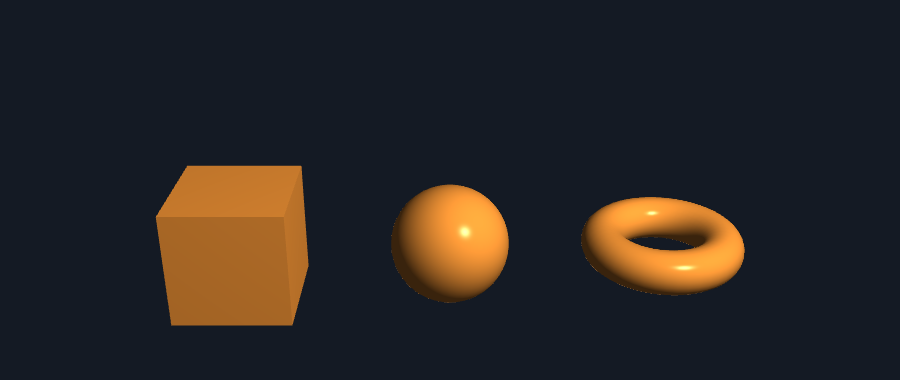
\includegraphics[width=\linewidth]{fig_light_default.png}\caption{Default light $(5,8,6)$}\end{subfigure}\hfill
\begin{subfigure}{0.49\textwidth}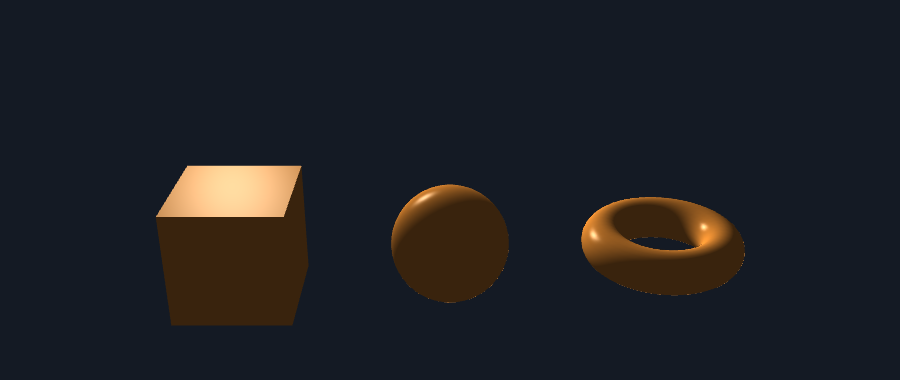
\includegraphics[width=\linewidth]{fig_light_moved.png}\caption{Light $(-3.34,3.89,-6.19)$}\end{subfigure}
\caption{Phong highlight on a flat face depends on the light position (same objects, same camera).}
\label{fig:light}
\end{figure}

\paragraph{Texture.} Images are loaded with \code{stb\_image} (rows flipped so that $v=0$ is the bottom), uploaded as RGBA8 with generated mipmaps, \code{GL\_REPEAT}
wrapping and trilinear filtering. A \emph{Tiling} slider multiplies the UV. If no image is chosen, a built-in checkerboard is used.

\begin{figure}[H]
\centering
\begin{subfigure}{0.48\textwidth}
\includegraphics[width=\linewidth]{fig_mode_flat.png}\caption{Flat color}\end{subfigure}\hfill
\begin{subfigure}{0.48\textwidth}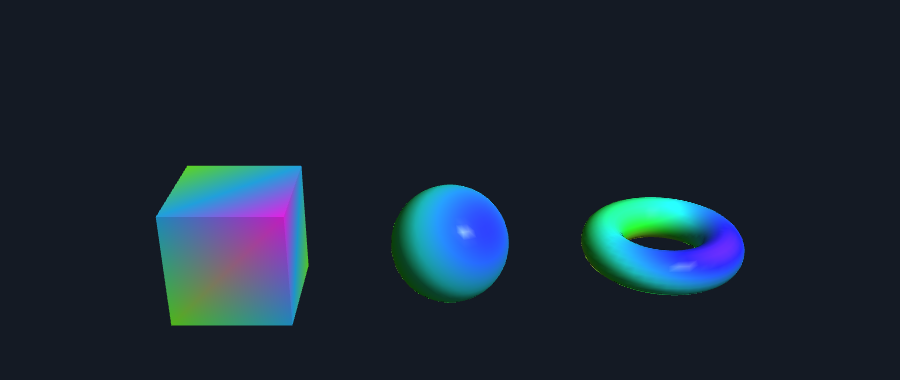
\includegraphics[width=\linewidth]{fig_mode_gouraud.png}\caption{Gouraud (rainbow vertex colors)}\end{subfigure}\\[4pt]
\begin{subfigure}{0.48\textwidth}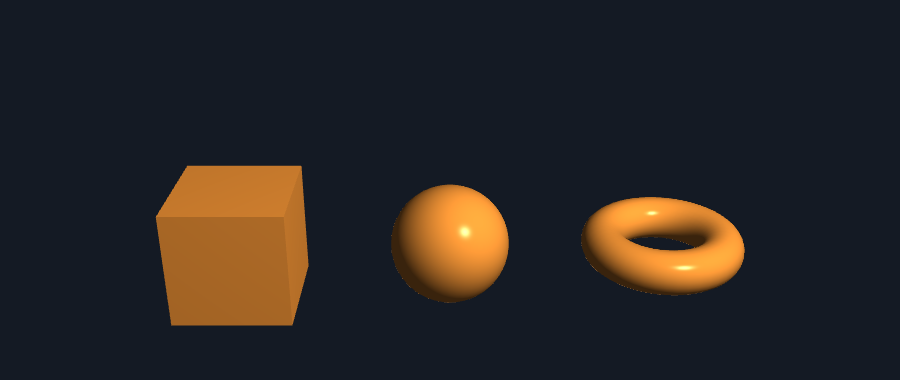
\includegraphics[width=\linewidth]{fig_mode_phong.png}\caption{Phong}\end{subfigure}\hfill
\begin{subfigure}{0.48\textwidth}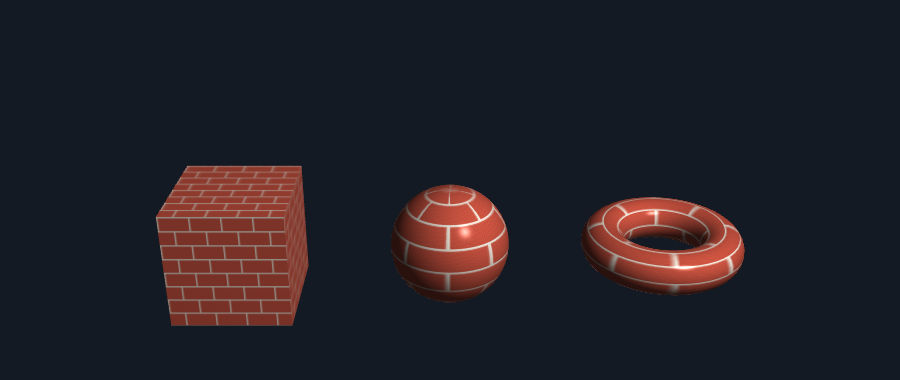
\includegraphics[width=\linewidth]{fig_mode_texture.png}\caption{Texture (bricks.png)}\end{subfigure}\\[4pt]
\begin{subfigure}{0.48\textwidth}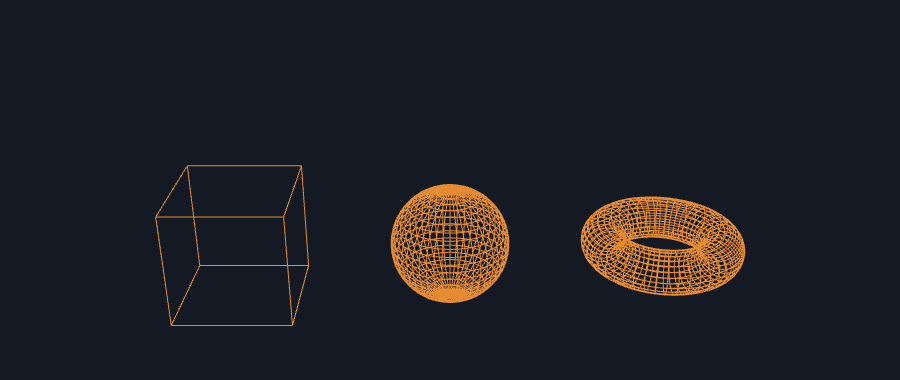
\includegraphics[width=\linewidth]{fig_mode_wire.png}\caption{Wireframe}\end{subfigure}
\caption{The five render modes on a cube, a sphere and a torus.}
\end{figure}

% ------------------------------------------------------------------ 6
\subsection{Object Transformations}\label{sec:transform}

Each object has a translation $t$, Euler rotation angles $(\theta_x,\theta_y,\theta_z)$ in degrees and a (non-uniform) scale $s$.
The model matrix is
\[
  M = T(t)\; R_z(\theta_z)\, R_y(\theta_y)\, R_x(\theta_x)\; S(s),
\]
i.e.\ a vertex is first scaled, then rotated about $X$, $Y$, $Z$ and finally translated. $M$ is uploaded as the \code{model} uniform, and
normals are transformed with the normal matrix $\bigl(M^{-1}\bigr)^{T}$ (upper $3\times3$), which stays correct under non-uniform scaling.
The inspector exposes these as sliders and shows the current $4\times4$ matrix. \emph{Ctrl\,+\,left drag} in the viewport rotates the selected object, and
\emph{Reset transform} returns it to the centre.

\subsection{User Interface and User Instructions}\label{sec:gui}

\subsubsection{Using the application}

\begin{figure}[H]
\centering
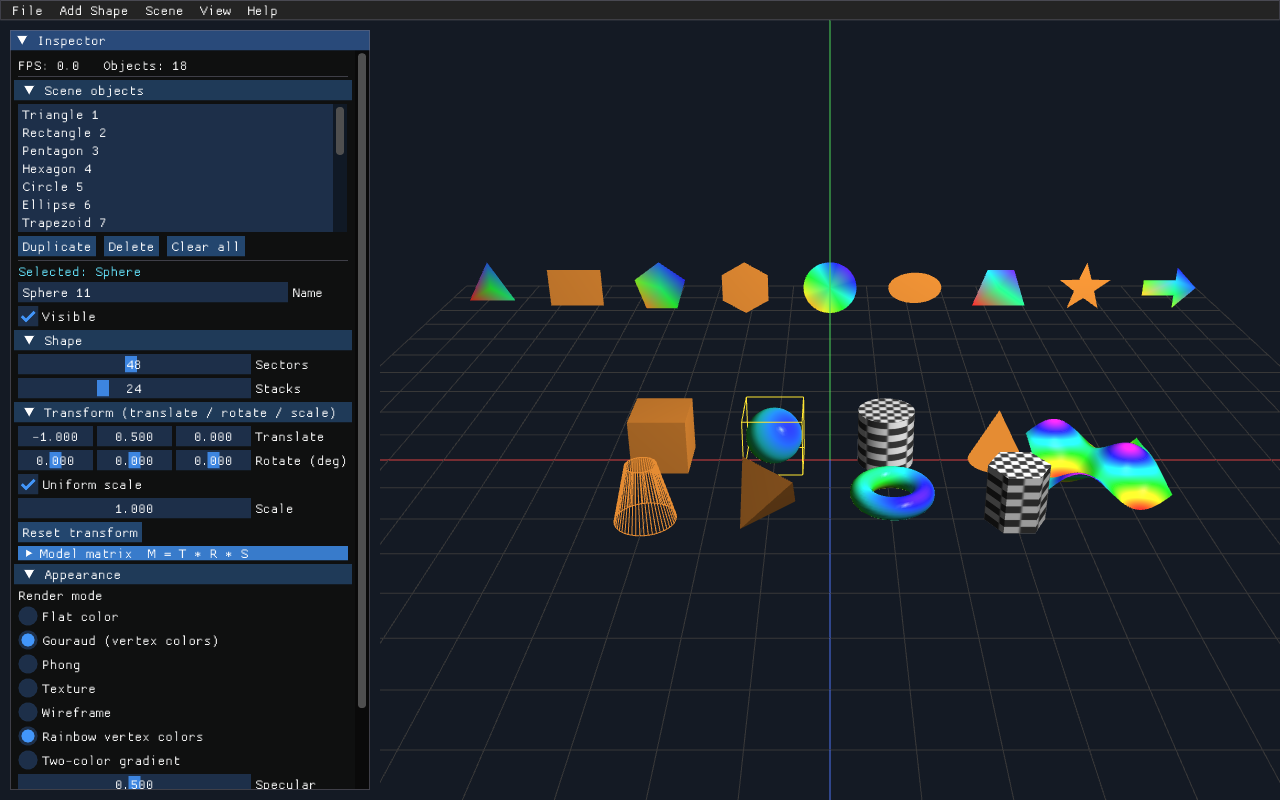
\includegraphics[width=\textwidth]{fig_gui.png}
\caption{The interface: menu bar (top), inspector (left) and the 3D viewport with the demo scene. The yellow box marks the selected object.}
\end{figure}

\begin{itemize}
  \item \textbf{Add Shape} menu: choose a 2D shape, a 3D shape, \emph{Surface $z=f(x,y)$} or \emph{Import model\ldots}. The new shape appears at the centre and becomes selected.
  \item \textbf{Inspector} $\rightarrow$ \emph{Scene objects}: select, duplicate, delete or clear objects. \emph{Shape}: parameters of the selected shape
        (segments, star points, inner ratio, top radius, tube radius, prism sides, rectangle size, \ldots). For a surface, the formula, presets, ranges and resolution.
  \item \emph{Transform}: translate / rotate / scale; \emph{Appearance}: render mode, color, specular and shininess, vertex-color scheme (Gouraud),
        texture image and tiling.
  \item \textbf{Scene} menu: delete / duplicate, clear, load a demo scene with all shapes, set all objects to one mode. \textbf{View} menu: reset camera, front (2D) view, top view, grid, axes.
        \textbf{File}: import a model, save a screenshot.
  \item \textbf{Lighting} (light position and colors) and \textbf{Camera / View} (field of view, distance, background) at the bottom of the inspector.
\end{itemize}

\begin{center}
\small
\begin{tabular}{@{}ll@{}}
\toprule
\textbf{Input} & \textbf{Action}\\
\midrule
Left mouse drag & orbit the camera\\
Right mouse drag & pan\\
Mouse wheel & zoom\\
Ctrl + left drag & rotate the selected object\\
Arrow keys / Shift + arrows & orbit / pan\\
\texttt{+} \texttt{-} or PageUp / PageDown & zoom\\
\texttt{R} & reset camera\\
\texttt{W} & toggle wireframe (selected object, or all if none is selected)\\
\texttt{Del} & delete the selected object\\
\texttt{F12} & save a screenshot (\texttt{screenshot\_<time>.png})\\
\texttt{H} / \texttt{Esc} & help window / quit\\
\bottomrule
\end{tabular}
\end{center}

\paragraph{Command line (for scripted screenshots).} All figures in this report were produced with options such as
\begin{verbatim}
./build/shapes --add star --add torus --mode phong --screenshot out.png
\end{verbatim}
{\raggedright Available options: \code{--demo}, \code{--add <shape>}, \code{--mode flat|gouraud|phong|texture|wire}, \code{--surface "<formula>"},
\code{--model <file>}, \code{--texture <png>}, \code{--view front|top}, \code{--distance d}, \code{--select i}, \code{--no-grid}, \code{--with-gui}.}

% ------------------------------------------------------------------ 7
\subsection{Results}

\begin{figure}[H]
\centering
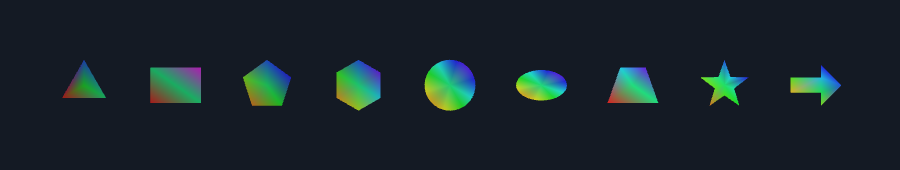
\includegraphics[width=\textwidth]{fig_2d.png}
\caption{2D shapes (front view, Gouraud with rainbow vertex colors): triangle, rectangle, pentagon, hexagon, circle, ellipse, trapezoid, star, arrow.}
\end{figure}

\begin{figure}[H]
\centering
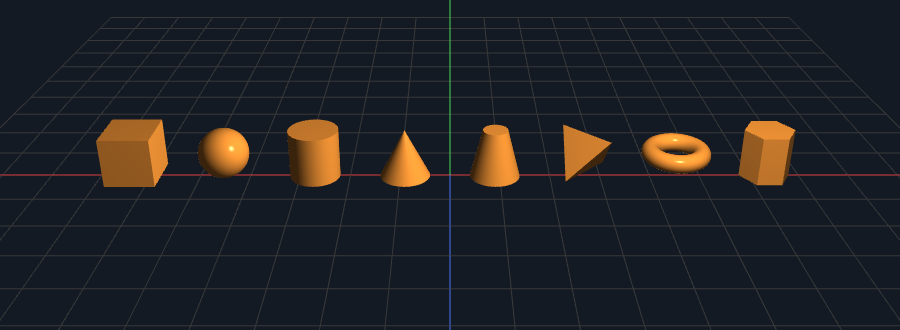
\includegraphics[width=\textwidth]{fig_3d.png}
\caption{3D solids (Phong): cube, sphere, cylinder, cone, truncated cone, tetrahedron, torus, prism.}
\end{figure}

\begin{figure}[H]
\centering
\begin{subfigure}{0.49\textwidth}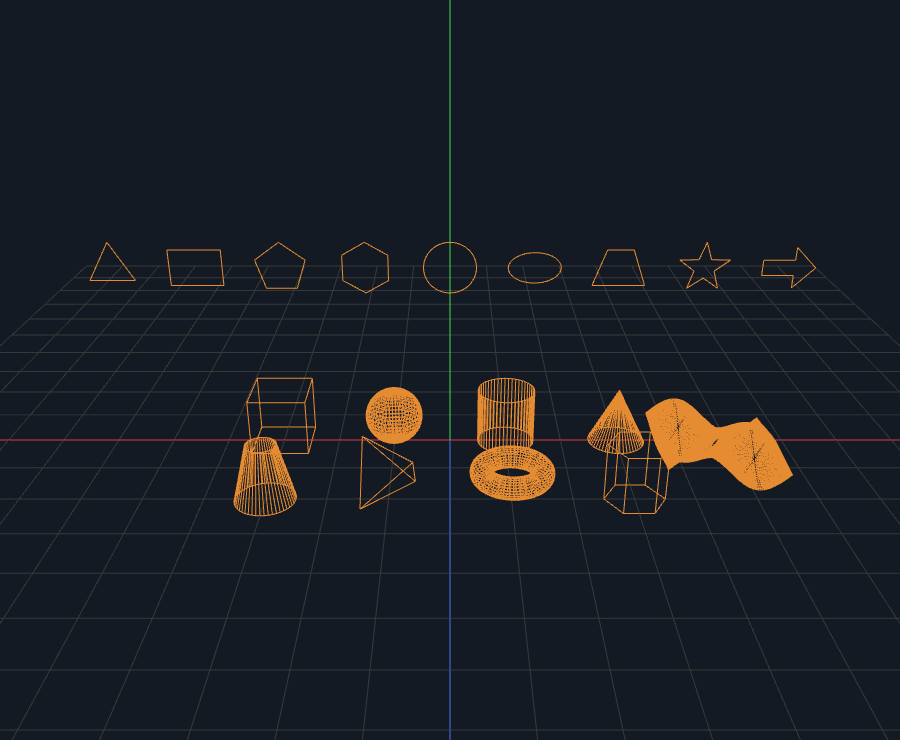
\includegraphics[width=\linewidth]{fig_wire.png}\caption{All shapes in wireframe: only the true edges}\end{subfigure}\hfill
\begin{subfigure}{0.49\textwidth}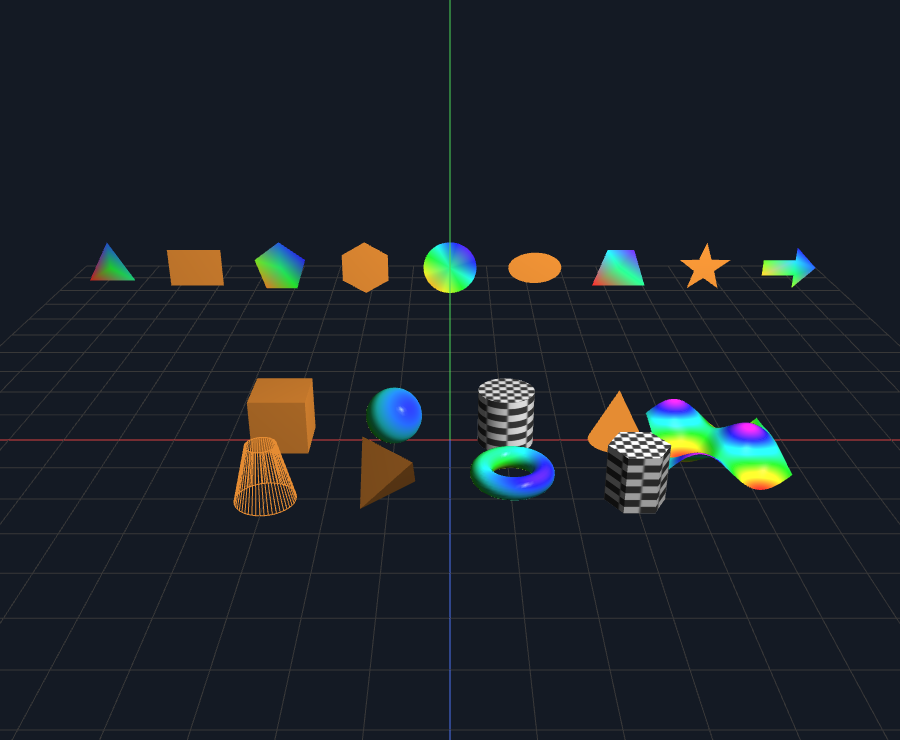
\includegraphics[width=\linewidth]{fig_demo.png}\caption{Demo scene: a mix of render modes}\end{subfigure}
\caption{Wireframe and mixed-mode scenes.}
\end{figure}

\begin{figure}[H]
\centering
\begin{subfigure}{0.49\textwidth}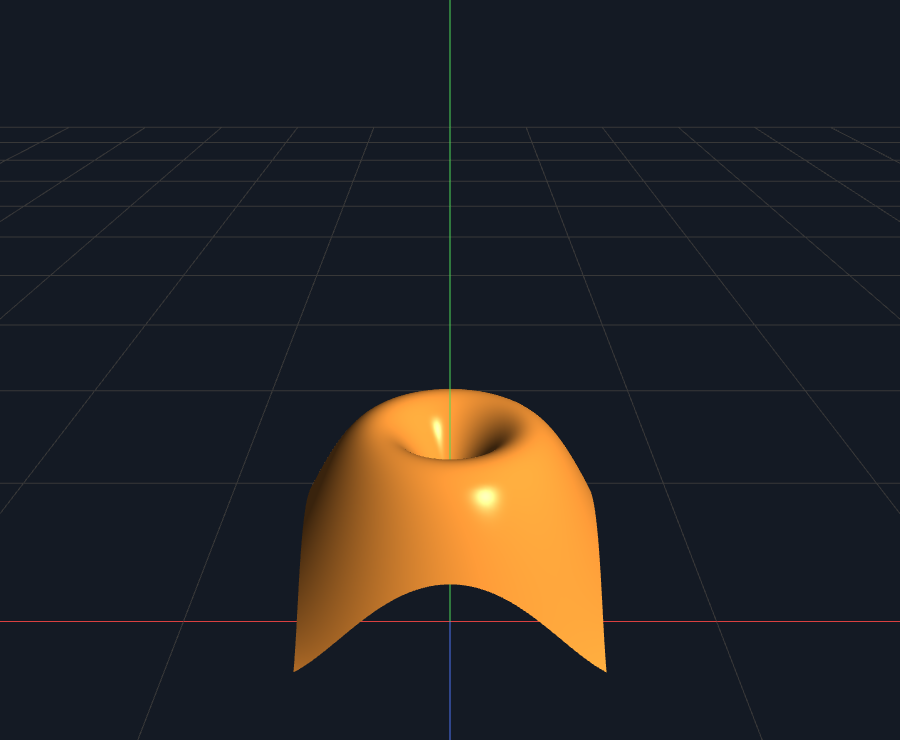
\includegraphics[width=\linewidth]{fig_surface.png}\caption{$z=2\sin\sqrt{x^2+y^2}$, range $[-3,3]^2$}\end{subfigure}\hfill
\begin{subfigure}{0.49\textwidth}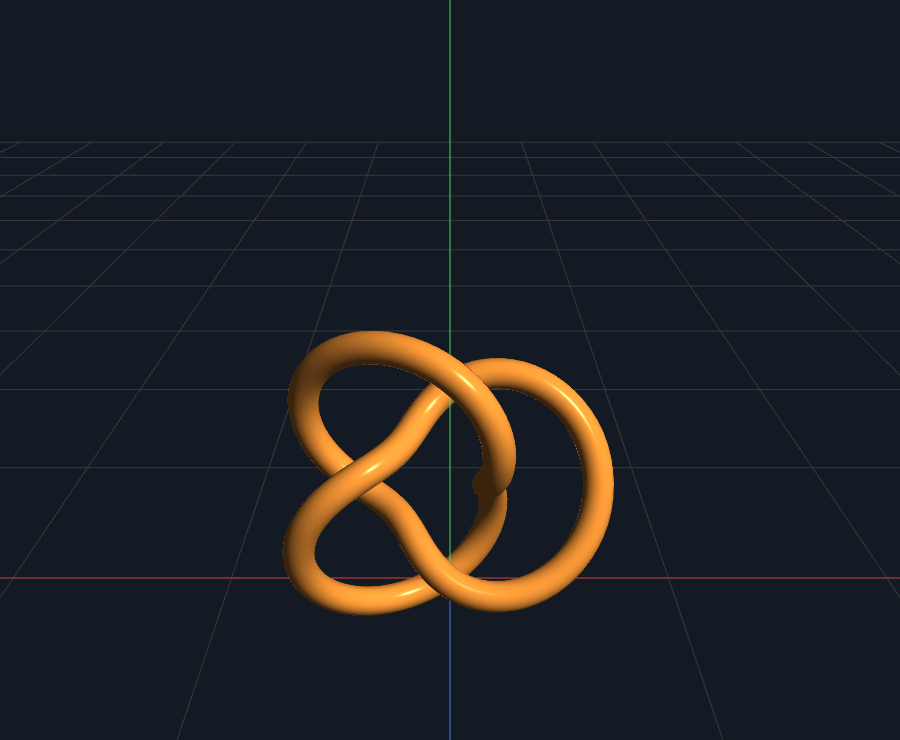
\includegraphics[width=\linewidth]{fig_model.png}\caption{Imported \texttt{torusknot.obj}}\end{subfigure}
\caption{A mathematical surface and an imported model, both in Phong mode.}
\end{figure}

\subsection{Testing}

\code{make test} builds \code{tests/test\_core.cpp}, which needs no GPU and checks:
\begin{itemize}
  \item the formula parser: precedence, right-associative power, unary minus, implicit multiplication, case-insensitivity, the \code{z=} prefix, and nine malformed
        inputs that must be rejected;
  \item every shape generator: all indices are in range, all normals are finite and unit length, colors are in $[0,1]$, the wire list is non-empty,
        every triangle is wound consistently with its normal (counter-clockwise from outside), and the exact number of edges of the planar shapes and solids
        (e.g.\ cube 12, hexagon 6, arrow 7, prism $3n$);
  \item surface building (valid, partly non-finite, fully non-finite, syntax error, empty range);
  \item the four sample models: loads correctly, is centred and fits a unit box, binary and ascii PLY, PLY colors preserved, missing file and unsupported extension rejected.
\end{itemize}
All 191\,199 checks pass. The closed-form counts of Table~\ref{tab:counts} were additionally verified against the generators by a separate program for all shapes at the defaults and for many
parameter combinations.


% ------------------------------------------------------------------ limitations
\subsection{Limitations}

ImGui has no native file dialog, so models and textures are chosen from the \code{assets/} folders or by typing a path; objects are selected from the list
(there is no picking by mouse click); OBJ faces are fan-triangulated, which assumes convex faces; material files (\code{.mtl}) are ignored; Gouraud shading interpolates the lit vertex
color, so highlights depend on mesh resolution (this is intended and shown in the comparison with Phong).

% ------------------------------------------------------------------ Part 2
\section{Part 2: Visualization of Atoms and Molecules}\label{sec:part2}

\subsection{Architecture and Components}

\subsection{Visualizing Atoms: Bohr's Model}

\subsection{Visualizing Molecules: Ball-and-Stick Model}

\subsection{Animation (Optional)}

\subsection{Rendering and Lighting}

\subsection{User Interface and User Instructions}

\subsection{Results}

\subsection{Limitations}

% ------------------------------------------------------------------ conclusion
\section{Conclusion}\label{sec:conclusion}

Both applications are built on the same OpenGL~3.3 core-profile foundation and on the shared code in \code{common/} (shader loading, orbit camera, ImGui, GLM), so
the two parts are independent programs that reuse the same graphics infrastructure.

\subsection{Part 1}
Part~1 draws all required 2D and 3D shapes, a user-defined surface and imported \code{.obj} / \code{.ply} models; supports the five render modes
(flat, Gouraud, Phong, texture, wireframe); lets the user translate, rotate and scale every object and navigate with mouse and keyboard; and is organised in small modules of which the geometry,
parsing and loading parts are independent from OpenGL and tested automatically.

\subsection{Part 2}

\section{Source Code}
\url{https://github.com/<account>/<repository>} (folders \code{part1\_shapes}, \code{part2\_molecules} and \code{common}).


% REFERENCES
\pagebreak
\begin{thebibliography}{9}
\addcontentsline{toc}{section}{References}
\bibitem{opengl33} M.~Segal and K.~Akeley, \emph{The OpenGL Graphics System: A Specification, Version 3.3 (Core Profile)}, Khronos Group.
\bibitem{phong} B.~T.~Phong, ``Illumination for Computer Generated Pictures,'' \emph{Communications of the ACM}, vol.~18, no.~6, pp.~311--317, 1975.
\bibitem{gouraud} H.~Gouraud, ``Continuous Shading of Curved Surfaces,'' \emph{IEEE Transactions on Computers}, vol.~C-20, no.~6, pp.~623--629, 1971.
\bibitem{glfw} GLFW -- an OpenGL library for windows, input and contexts. \url{https://www.glfw.org}
\bibitem{glew} GLEW -- the OpenGL Extension Wrangler Library. \url{https://glew.sourceforge.net}
\bibitem{glm} G-Truc Creation, OpenGL Mathematics (GLM). \url{https://github.com/g-truc/glm}
\bibitem{imgui} O.~Cornut, Dear ImGui -- bloat-free graphical user interface for C++. \url{https://github.com/ocornut/imgui}
\bibitem{stb} S.~Barrett, stb single-file public domain libraries (\code{stb\_image}, \code{stb\_image\_write}). \url{https://github.com/nothings/stb}
\end{thebibliography}

\end{document}
